\section{Preliminaries}
\subsection{LZ compression}
\label{subsection:LZCompression}
The most important part in LZ-Index \cite{LZIndex} is the fact that we want to search for patterns within the compressed text. The compressions that can be used for this particular structure are LZ78 \cite{LZ78} and LZW \cite{LZW}. Here we will focus on the LZ78 compression. 

\subsubsection{Idea of LZ78 compression}

The main idea of LZ78 compression is to convert text $t$ into sequence of blocks, where the block will be in form $(i, c)$ where $i$ is an index and $c$ is the character of $t$, so the output of the LZ78 compression will be a sequence of $B_1,...,B_w$. Each of the block will clearly represent some substring of $t$ and after translating this block to that substring we will get exactly text $t$. The  block $B_x$ is defined as a pair $(i, c)$ such that $B_x$ correspond to the string obtained from decompressing $B_i$ adding character $c$ at the end or just $c$ if $i = 0$. So we will use the previous blocks to create a new one by extending them with one character, so the idea can be written as:

\begin{enumerate}
    \item Start with the empty string $q$ and previous block as $prev$ = 0.
    \item Get next character $c$ of $t$.
    \item If there is no block that represents string $q + c$ or $c$ is last character of $t$, then add to result block $(prev, c)$, set $prev = 0$ and go to step 3.
    \item Otherwise, which means that there is a block $B_z$, that it represents string $q + c$, set $prev = z$ and go to step 3.
\end{enumerate}

To summarize it with one sentence: get next character of $t$ and add it to current string, if it is unique at that moment create a new block from the previous one and start again from empty string with next character of $t$.

\subsubsection{Example of LZ78 compression}

Let's try to find a LZ78 compression of text $t = aabb$. We start with:

\begin{table}[H]
\begin{center}
\begin{tabular}{|c|c|c|c|c|}
\hline
\rowcolor[HTML]{C0C0C0} 
step  & result & current string & previous block & blocks mapping \\ \hline
0                 & {[} {]} & ' '             & 0              & \{\}           \\ \hline
\end{tabular}

\end{center}
\end{table}
Going forward with loop the next character is $a$.

\begin{table}[H]
\begin{center}
\begin{tabular}{|c|c|c|c|c|}
\hline
\rowcolor[HTML]{C0C0C0} 
step & result  & current string & previous block & blocks mapping \\ \hline
0                & {[} {]} & ' '            & 0              & \{\}           \\ \hline
1               & {[} {]} & 'a'            & 0              & \{\}           \\ \hline
\end{tabular}
\end{center}
\end{table}
There is no block that correspond to the string currently under consideration so we add new block, set default values and look at the next character.

\begin{table}[H]
\begin{center}
\begin{tabular}{|c|c|c|c|c|}
\hline
\rowcolor[HTML]{C0C0C0} 
step  & result         & current string & previous block & blocks mapping   \\ \hline
0               & {[} {]}        & ' '            & 0              & \{\}             \\ \hline
1              & {[} {]}        & 'a'            & 0              & \{\}             \\ \hline
2             & {[} (0, a) {]} & 'a'            & 0              & \{ $B_1$ = 'a' \} \\ \hline
\end{tabular}
    
\end{center}
\end{table}
There is already a block that correspond to string $'a'$, so we continue with the next character.

\begin{table}[H]
\begin{center}
\begin{tabular}{|c|c|c|c|c|}
\hline
\rowcolor[HTML]{C0C0C0} 
Step & result         & current string & previous block & blocks mapping   \\ \hline
0    & {[} {]}        & ' '            & 0              & \{\}             \\ \hline
1    & {[} {]}        & 'a'            & 0              & \{\}             \\ \hline
2    & {[} (0, a) {]} & 'a'            & 0              & \{ $B_1$ = 'a' \} \\ \hline
3    & {[} (0, a) {]} & 'ab'           & 1              & \{ $B_1$ = 'a' \} \\ \hline
\end{tabular}
  
\end{center}
\end{table}
Now string currently under consideration is unique withing current mapped blocks, so we add it as a new block and goes with new character.

\begin{table}[H]
\begin{center}
\begin{tabular}{|c|c|c|c|c|}
\hline
\rowcolor[HTML]{C0C0C0} 
step & result                 & current string & previous block & blocks mapping                \\ \hline
0    & {[} {]}                & ' '            & 0              & \{\}                          \\ \hline
1    & {[} {]}                & 'a'            & 0              & \{\}                          \\ \hline
2    & {[} (0, a) {]}         & 'a'            & 0              & \{ $B_1$ = 'a' \}              \\ \hline
3    & {[} (0, a) {]}         & 'ab'           & 1              & \{ $B_1$ = 'a' \}              \\ \hline
4    & {[} (0, a), (1, b) {]} & 'b'            & 0              & \{ $B_1$ = 'a', $B_2$ = 'ab' \} \\ \hline
\end{tabular}
   
\end{center}
\end{table}
The last character is $b$ which is also unique string, so the result of compression will be $(0, a), (1, b), (0, b)$.


\subsubsection{Properties of LZ78 compression}

Let us start by stating some interesting properties of the LZ78 compression.

\begin{observation} \cite{LZIndex} 
    Let $B_1,...,B_w$ be the LZ78 compression of $t$. Each of these blocks is unique, possibly except the last one. We can make them all unique appending to $t$ a character that does not appear in the alphabet.
\end{observation}

\begin{proof}
    Let us prove it by contradiction. Let us assume that there are two blocks $B_i, B_j$ such that $B_i = B_j$, $1 \leq i \neq j < w$. Without loss of generality we assume that $j > i$. Taking into consideration LZ78 compression algorithm. If there already exists the block that is representing the same substring, we are considering the next character of $t$, so we cannot add that block to the result. From the fact that $i, j < w$, none of the blocks $B_i, B_j$ is the last one block, so the next character always exists. That implies that such situation cannot happen. Appending the character that does not appear in the alphabet, we ensure that the last one block is unique, because such character is already unique in $t$.
\end{proof}

The above observation is essential in LZ-index pattern searching procedure, we will need all the blocks to be unique. 

\begin{observation} \cite{LZ78} 
    LZ78 is a lossless compression, that is, it can be decompressed unambiguously, to obtain text $t$.
\end{observation}

That observation can be easily by contradiction straight form the decompressing procedure.

\begin{observation} \cite{entropyProof}
    In the worst case LZ78 compression will use $x + o(x)$ bits, where $x$ is a number of bits of uncompressed text.
\end{observation}

\begin{observation} \cite{entropyProof} 
    The compression rate of LZ78 compression in average case asymptotically approaches to entropy of text $t$.
\end{observation}

Proof of above observation is quite complicated and requires advanced knowledge of probability, so it won't be discussed here. 


\subsection{LZTrie}
The first structure required for LZ-Index is LZTrie. It is a tree consisting of all blocks of LZ78 compression, where each node correspond to a single block of compressed text. By creating that structure you can also compress the text at once, like in the compression procedure presented above. The only difference in this case is that all blocks are represented as nodes. That structure has to permit the following operations for each node:

\begin{itemize}
    \item $\texttt{id(x)}$ -- returns the identifier of block which can be just an index of the block in compressed text.
    \item $\texttt{children(x)}$ -- computes a structure that holds all the children of given node. The returned collection has to answer fast for query like $\texttt{child(c)}$ which should return a child of $x$ such that string represented by $x$ is extended by character $c$ in that child or recognize that such child not exist.
    \item $\texttt{parent(x)}$ -- provides the parent of given node.
    \item $\texttt{depth(x)}$ -- retrieves the depth of given node counted from the root of the tree. It will be used to count the offset for pattern beginning index.
    \item $\texttt{rank(x)}$ -- returns the rank of given node in lexicographic order.
    \item $\texttt{position(x)}$ -- returns a position in which given node begins in uncompressed text. It is used for mapping the raw result of string-searching performed on LZ-Index, which is a set of pairs $(i, j)$, where $i$ is the index of a block in compressed text and $j$ is the offset for the beginning of that block.
    \item $\texttt{left\_rank(x)}$ and $\texttt{right\_rank(x)}$ -- retrieves the minimum and maximum rank of proper node in given node subtree.
\end{itemize}
The LZTrie structure has to perform search for given string that will return the node which represents that string in LZTrie. 

\begin{center}
    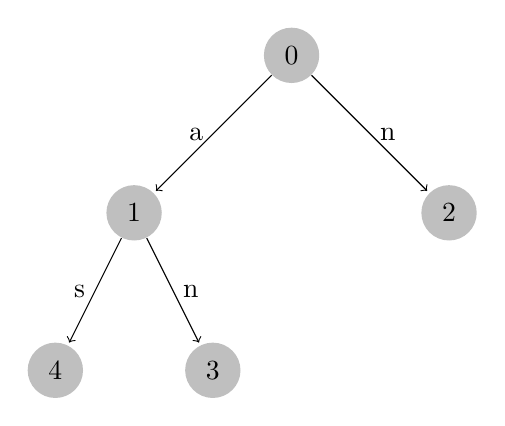
\begin{tikzpicture}[shorten >=1pt,->]
      \tikzstyle{vertex}=[circle,fill=black!25,minimum size=20pt,inner sep=4pt]
      \node[vertex] (G_1) at (-2,-2) {1};
      \node[vertex] (G_2) at (0,0)   {0};
      \node[vertex] (G_3) at (2,-2)  {2};
      \node[vertex] (G_4) at (-1,-4)  {3};
      \node[vertex] (G_5) at (-3,-4)  {4};
      \draw[] (G_2) -- (G_1) node [midway, left] {a};
      \draw[] (G_2) -- (G_3) node [midway, right] {n};
      \draw[] (G_1) -- (G_4) node [midway, right] {n};
      \draw[] (G_1) -- (G_5) node [midway, left] {s};
    \end{tikzpicture}
    \captionof{figure}{Example LZTrie for $t = ananas$}
\end{center}

The creation of LZTrie node and also RevLZTrieNode can be implemented in the following way:

\begin{minted}[xleftmargin=20pt, linenos]{python}
class _LZTreeNode:
  def __init__(self, parent, character, idx, position):
    self.parent = parent
    self.position = position
    if parent is not None:
      parent.children[character] = self
      self.depth = parent.depth + 1
    else:
      self.depth = 0
    self.idx = idx
    self.children = {}
    self.character = character
    self.rank = None
    self.left_rank = None
    self.right_rank = None
\end{minted}

For proper setting $rank$, $left\_rank$, $right\_rank$ properties we have to build the whole tree and then traverse it, so it requires separate function:

\begin{minted}[xleftmargin=20pt, linenos]{python}
  def set_ranks(self, rank):
    if self.idx is not None:
      self.rank = rank
      self.left_rank = rank
      self.right_rank = rank
      rank = rank + 1
    if len(self.children) > 0:
      for child_key in sorted(self.children):
        rank = self.children[child_key].set_ranks(rank)
      min_key = min(self.children)
      max_key = max(self.children)
      self.left_rank = (self.children[min_key].left_rank
        if (self.rank is None or
          self.children[min_key].left_rank < self.rank)
        else self.rank)
      self.right_rank = (self.children[max_key].right_rank
        if (self.rank is None or
          self.children[max_key].right_rank > self.rank)
        else self.rank)
    return rank
\end{minted}

As for implementation of construction the LZTrie it looks just like the compression algorithm mentioned in \Cref{subsection:LZCompression}.

\begin{minted}[xleftmargin=20pt, linenos]{python}
class _LZTrie:
  def __init__(self, t, n):
    t += '$'
    self.root = _LZTreeNode(None, '#', 0, None)
    current_node = self.root
    index, position = 1, 1
    for i in range(1, n+2):
      current_char = t[i]
      if current_char not in current_node.children:
        _LZTreeNode(current_node, current_char, idx, position)
        index += 1
        current_node = self.root
        position = i+1
      else:
        current_node = current_node.children[current_char]
    self.size = index
    self.root.set_ranks(0)

def search(tree, t, n):
  return _search_private(t, 0, n, tree.root)

def _search_private(tree, index, n, node):
  if index == n:
    return node
  if tree[index+1] not in node.children:
    return None
  return _search_private(tree, index+1, n, node.children[tree[index+1]])
\end{minted}

LZTrie creation requires $\bigO(n \cdot \log (|\mathcal{A}|))$ time for a given text of length $n$.

\subsection{RevLZTrie}
RevLZTrie structure behaves like LZTrie, but there are some differences. The first one is that the RevLZTrie is created by passing each node of LZTrie and going from it to the root. Formally, it is created by reversed strings of compressed text and not by passing the reversed text to LZTrie. The RevLZTrie consists of the same types of nodes as LZTrie so each of them can perform the same operations. The main difference is that in RevLZTrie there are some nodes that do not correspond to any blocks of the compressed text, so the size of that structure can be equal to the length of uncompressed text, but still the complexity of creation it is exactly the same as for LZTrie which is $\bigO(n \cdot \log (|\mathcal{A}|))$. 
\begin{center}
    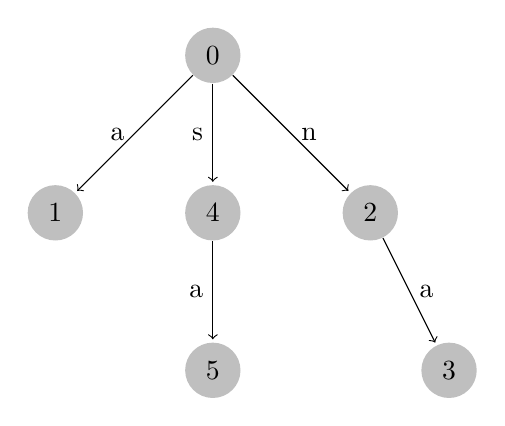
\begin{tikzpicture}[shorten >=1pt,->]
      \tikzstyle{vertex}=[circle,fill=black!25,minimum size=20pt,inner sep=4pt]
      \node[vertex] (G_1) at (-2,-2) {1};
      \node[vertex] (G_2) at (0,0)   {0};
      \node[vertex] (G_3) at (2,-2)  {2};
      \node[vertex] (G_4) at (3,-4)  {3};
      \node[vertex] (G_5) at (0,-2)  {4};
      \node[vertex] (G_6) at (0,-4)  {5};
      \draw[] (G_2) -- (G_1) node [midway, left] {a};
      \draw[] (G_2) -- (G_3) node [midway, right] {n};
      \draw[] (G_3) -- (G_4) node [midway, right] {a};
      \draw[] (G_2) -- (G_5) node [midway, left] {s};
      \draw[] (G_5) -- (G_6) node [midway, left] {a};
    \end{tikzpicture}
    \captionof{figure}{RevLZTrie for LZTrie from Figure 3.1}
\end{center}

The example implementation looks like this:

\begin{minted}[xleftmargin=20pt, linenos]{python}
class _RevLZTrie:
  def __init__(self, lz_trie):
    self.root = _LZTreeNode(None, '#', 0, None)
    self._add_recursive(lz_trie.root)
    self.root.set_ranks(0)

  def _add_recursive(self, node):
    for child in node.children.values():
      self._add_recursive(child)
      self._add_block(child, self.root, child.idx)

  def _add_block(self, lz_node, rev_node, idx):
    if lz_node.parent is None or lz_node.parent.character == '#':
      if lz_node.character in rev_node.children:
        rev_node.children[lz_node.character].idx = idx
      else:
        rev_node.children[lz_node.character] = (_LZTreeNode(rev_node,
          lz_node.character, idx, None))
    else:
      if lz_node.character not in rev_node.children:
        rev_node.children[lz_node.character] = (_LZTreeNode(rev_node,
          lz_node.character, None, None))
      self._add_block(lz_node.parent,
        rev_node.children[lz_node.character], idx)
\end{minted}

Note that $\texttt{search(tree, n, root)}$ function works properly for both LZTrie and RevLZTrie.

\subsection{Range structure}
One of the structures needed for LZ-index is a structure that can perform two-dimensional searching in space $[0, n] \times [0,n]$.

\begin{problem}[Two-dimensional search in space $\lbrack0, n\rbrack \times \lbrack0,n\rbrack$]
Given a set of points $P = \{ (x, y): x \in \lbrack0, n\rbrack, y \in \lbrack0, n\rbrack \}$ of size $m$. For each query of form $[l_1, r_1]$, $[l_2, r_2]$ return all points from $P$ that $x \in [l_1, r_1]$ and $y \in [l_2, r_2]$.
\end{problem}

There are many ways to solve that problem, the first one is naive approach which for each point $p \in P$ checks if it fulfills condition from the query. Such approach is very simple and will work in $\bigO(m)$ time as for each point we need constant time to check the query condition, but it can be done faster. First, we sort the points by their first coordinate. Then, we create Wavelet Tree from the list of second coordinates from sorted points. With such preprocessing, we can now answer queries by performing two binary searches to first find the indices $l, r$ such that all points in range $[l, r]$ fulfills search condition for first coordinate, and then we use $\texttt{range\_search(l, r, x, y)}$ function for Wavelet Tree with arguments $l$, $r$, $l_2$, $r_2$ and maps the result. Note that the result of $\texttt{range\_search(l, r, x, y)}$ is exactly the list of all indices for points that fulfil the condition for first and second coordinate. Implementation of that structure can be done in the following way:

\begin{minted}[xleftmargin=20pt, linenos]{python}
class _RangeSearcher:
  def __init__(self, points):
    self.points = sorted(points, key= lambda x: x[0])
    values = ['#'] + [y for x, y in self.points]
    self.wavelet_tree = wavelet_tree.WaveletTree(values, len(values)-1)

  def search_in_range(self, l1, r1, l2, r2):
    l, r = 0, len(self.points)
    while l < r:
      s = (l+r)//2
      x, _ = self.points[s]
      if x < l1:
        l = s+1
      else:
        r = s
    left = l
    l, r = -1, len(self.points)-1
    while l < r:
      s = (l+r+1)//2
      x, _ = self.points[s]
      if x <= r1:
        l = s
      else:
        r = s-1
    right = l
    if left > right or left == len(self.points) or right == -1:
      return []
    return ([self.points[x-1] for x in
              self.wavelet_tree.range_search(left+1, right+1, l2, r2)])
\end{minted}

Time needed for construction RankSearcher is equal to $\bigO(m \log m)$ due to the sorting and the creation of Wavelet Tree. Moreover, answering the query use only $\bigO(R\cdot \log(m) + \log(m))$ time, where $R$ is the number of points that are returned from query. The input for creation of RangeSearcher will be all pairs in form $(B_i.rev\_rank, B_{i+1}.rank)$ for all $i$ less than number of block in compressed text and where $B_i.rev\_rank$ is the rank if $i$-th block in RevLZTrie.

\subsection{NodeMapper structure}
The NodeMapper structure retrieves node of RevLZTrie that represents a block at the given index in LZ78 compression. Such structure can be created by using information from RevLZTrie nodes and just all of them in any order. It requires $\bigO(n)$ time due to the fact that some nodes of RevLZTrie does not represent any block of compressed text.

\begin{minted}[xleftmargin=20pt, linenos]{python}
class _NodeMapper:
  def __init__(self, lz_trie, size):
    self.arr = [None] * size
    self._map_tree_to_list(lz_trie.root)

  def _map_tree_to_list(self, node):
    if node.idx is not None:
      self.arr[node.idx] = node
    for child in node.children.values():
      self._map_tree_to_list(child)

  def get_node_by_idx(self, idx):
    return self.arr[idx]
\end{minted}

The creation of this structure requires to visit all $\bigO(n)$ nodes of RevLZTrie, and the query requires $\bigO(1)$ time. This structure is also used for receiving the text position from blocks, so it also has to be build for LZTrie.

\subsection{RankMapper structure}
The last structure we need to perform string-searching in LZ78 compressed text is called RankMapper. That structure allows us to find the $i$-th node in lexicographical order. That structure has to be build for both LZtrie and RevLZTrie, but it can be also done in simple way using the idea already invoked for the creation of NodeMapper. To build RankMapper one can just visit all the nodes of the tree and set their index in a suitable array, as presented below:

\begin{minted}[xleftmargin=20pt, linenos]{python}
class _RankMapper:
  def __init__(self, lz_trie, size):
    self.arr = [None] * size
    self._map_tree_to_list(lz_trie.root)

  def _map_tree_to_list(self, node):
    if node.rank is not None:
      self.arr[node.rank] = node
    for child in node.children.values():
      self._map_tree_to_list(child)

  def get_node_by_rank(self, rank):
    return self.arr[rank]
\end{minted}

The complexity of creation RankMapper and performing a query is exactly the same as for NodeMapper. Having all of that structures in hand, LZ-Index can be constructed as follows:

\begin{minted}[xleftmargin=20pt, linenos]{python}
class _LZIndex:
  def __init__(self, lz_trie, rev_lz_trie, lz_node_mapper, 
        rev_lz_node_mapper, range_searcher, lz_rank_mapper, 
        rev_lz_rank_mapper):
    self.lz_trie = lz_trie
    self.rev_lz_trie = rev_lz_trie
    self.lz_node_mapper = lz_node_mapper
    self.range_searcher = range_searcher
    self.rev_lz_node_mapper = rev_lz_node_mapper
    self.lz_rank_mapper = lz_rank_mapper
    self.rev_lz_rank_mapper = rev_lz_rank_mapper

def create_lz_index(t, n):
  lz_trie = _LZTrie(t, n)
  rev_trie = _RevLZTrie(lz_trie)
  lz_node_mapper = _NodeMapper(lz_trie, lz_trie.size)
  rev_node_mapper = _NodeMapper(rev_trie, lz_trie.size)

  points = [(rev_node_mapper.get_node_by_idx(i).rank,
    lz_node_mapper.get_node_by_idx(i+1).rank)
    for i in range(1, lz_trie.size - 1)]
  range_searcher = _RangeSearcher(points)
  lz_rank_mapper = _RankMapper(lz_trie, lz_trie.size)
  rev_lz_rank_mapper = _RankMapper(rev_trie, lz_trie.size)
  return _LZIndex(lz_trie, rev_trie, lz_node_mapper, rev_node_mapper,
    range_searcher, lz_rank_mapper, rev_lz_rank_mapper)
\end{minted}



